% Changing book to article will make the footers match on each page,
% rather than alternate every other.
%
% Note that the article class does not have chapters.
\documentclass[letterpaper,10pt,twoside,twocolumn,openany]{book}

% Use babel or polyglossia to automatically redefine macros for terms
% Armor Class, Level, etc...
% Default output is in English; captions are located in lib/dndstring-captions.sty.
% If no captions exist for a language, English will be used.
%1. To load a language with babel:
%   \usepackage[<lang>]{babel}
%2. To load a language with polyglossia:
%   \usepackage{polyglossia}
%   \setdefaultlanguage{<lang>}
\usepackage[english]{babel}
%usepackage[italian]{babel}
% For further options (multilanguage documents, hypenations, language environments...)
% please refer to babel/polyglossia's documentation.

\usepackage[utf8]{inputenc}
\usepackage{lipsum}
\usepackage{listings}
\usepackage{float}
\usepackage{wrapfig}
%\usepackage{tikz}

% dnd package options 
% bg-full   : Default option. Use paper background and fancy footer.
% bg-print  : Use fancy footer but not background.
% bg-none   : No paper background and plain footer.
% justified : Use full justification for text layout instead of ragged right.
\usepackage{dnd}

\lstset{%
  basicstyle=\ttfamily,
  language=[LaTeX]{TeX},
}

\title{Underdark}
\author{ocket8888}

\usepackage{eso-pic}
\newcommand\BackgroundPic{%
\put(0,0){%
\parbox[b][\paperheight]{\paperwidth}{%
\vfill
\centering
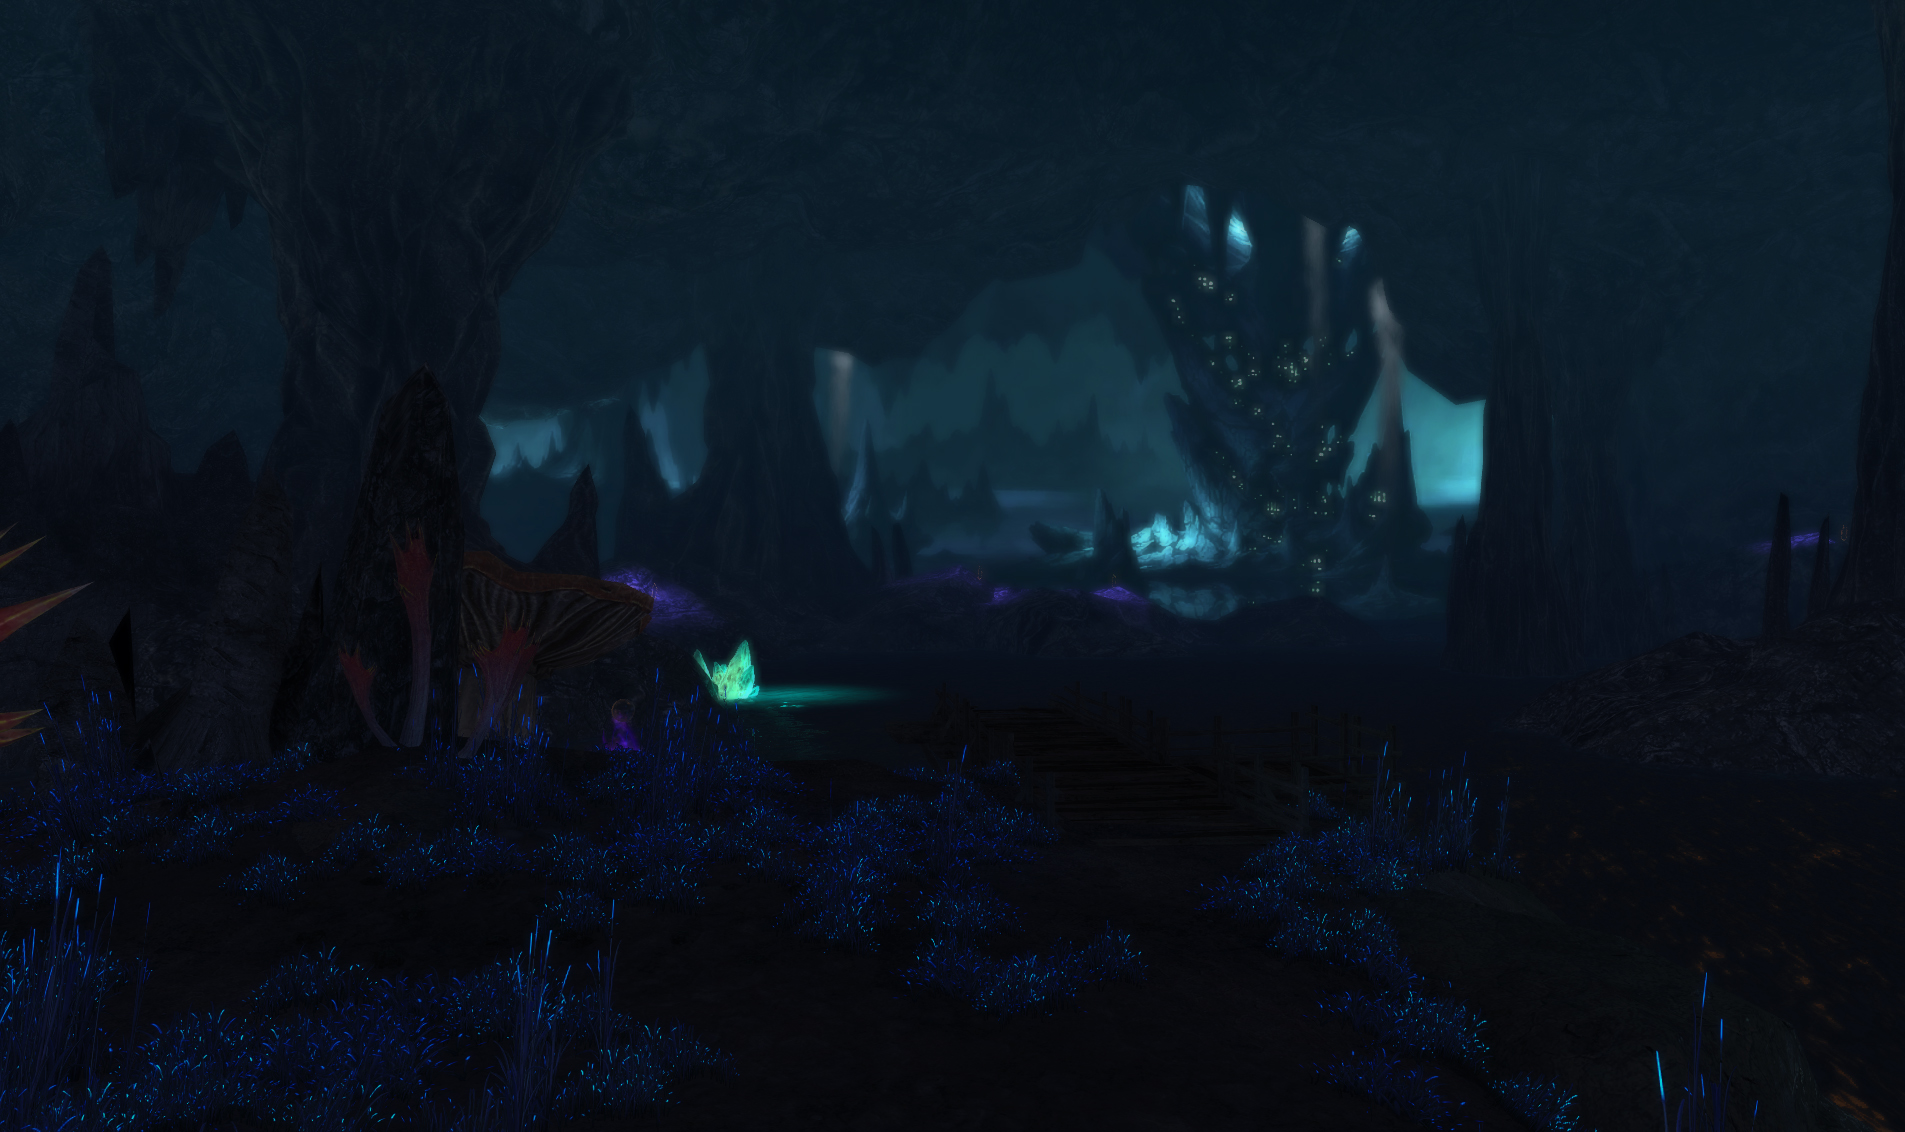
\includegraphics[width=\paperwidth,height=\paperheight]{img/dist/underdark.jpg}%
\vfill
}}}

\usepackage[pdfusetitle,
			pdfsubject={Fantasy},
			pdfkeywords={Dungeons and Dragons, Roleplaying, Fantasy, Adventure},
			pdfproducer={MikTeX},
			pdfcreator={XeLaTeX}]{hyperref}

\usepackage{fontspec}
\usepackage{caption}
\usepackage{xunicode}

\defaultfontfeatures{Mapping=tex-text}
\newfontfamily\figcapfont{Zapfino}% Some other font
\DeclareCaptionFormat{figcapfont}{\figcapfont #1#2#3}
\captionsetup[figure]{format=figcapfont}
\setmainfont{ScalaSans}
\setsansfont{DungeonFixed}% Based on the Dungeon font (filename "DUNGRG__.ttf"), with added glyphs for single right quote and right-left double quotes
\titleformat*{\chapter}{\Huge\sffamily}


\pagestyle{fancy}
\thispagestyle{plain}

% Start document
\begin{document}
\AddToShipoutPicture*{\BackgroundPic}%Yeezus this was difficult
\begin{titlepage}
\centering

\includegraphics[width=0.5\paperwidth,keepaspectratio]{img/dist/title.pdf}\\
{\Large \color{white} \textasciitilde{} The Captive Chronicles Pt. 1 \textasciitilde}
\end{titlepage}

\chapter*{Introduction}
Deep beneath the surface of the world lies the Underdark. a realm of endless labyrinthine tunnels and caverns where the Sun never shines. The Underdark is filled with races and creatures too numerous to count or list, and foremost among these are the dark elves- the Drow. Hated and feared even by their fellow dwellers in darkness, the Drow raid other settlements in the Underdark as well as the surface world, taking prisoners back with them. Rendered unconscious with Drow poison, then collared and shackled, these prisoners are eventually sold as slaves or entertainment in the dark elves' subterranean cities. 

Our adventurers have all had the misfortune of falling to such a fate. Captured by the Drow, they are prisoners at one of the Drow's outposts awaiting transport to the great slave city of Menzobarranzan, the city of spiders.

\chapter{1. Captive}
In the suffocating, malodorous dark of large cell in the Drow outpost's prison, a scheme was being formulated. The man doing the scheming, a tall Wood Elf in his mid 20's with short, messy, chestnut colored hair and emerald eyes, was named Dox Evenwood, and he felt that he and his companion Jhank had spent far too long in the cell already. Jhank was a hulking 7' Lizardman, with olive-green scales and a bright orange/yellow fin protruding from the top of his head to about his shoulder blades. Both were frustrated with their situation, but Jhank was approaching furious.\\

The cell in which the prisoners found themselves was quite large, and contained numerous exotic beings. By the dim, flickering torchlight, one can just make out the rocky walls of the enclosure, one of which played host to a row of chamberpots that the prisoners were made to empty each day by flinging their contents over the side of a gaping abyss just outside the cell doors. The rush of water could be heard faintly, as a waterfall poured over the side into fathomless black.\\

With the recent arrivals, Dox felt confident an escape attempt was within their grasp. Already incarcerated upon their arrival was a host of interesting and potentially instrumental characters. The more resourceful among them had begun to squirrel away items that might prove useful in an escape attempt. Dox himself had acquired a crossbow which carried an odd smell, and Jhank had procured a heavy, solid bar of metal.\\

Most unusual among them was what appeared to be a huge mushroom that stumbled around the cell on stumpy legs. It stood approximately 3.5 feet tall, and seemed to move back and forth somewhat fretfully, avoiding other prisoners. Occasionally, it would emit a puff of reddish particulate into the air from its cap. Prisoners have noticed that standing near the mushroom-man caused them to hear voices in their head, saying things such as "...the grove remembers..." and "...must return to the others...".

Another of the more reclusive prisoners was a large, pensive toad-like creature that seemed content to pass its time sitting by a wall. The fish-man rocked back and forth and periodically issued guttural noises from deep within its throat. Despite the somewhat threatening size of the fish-man and the low, growl-like noises he was making, he appeared to be quite approachable, looking at those who passed nearby with a sort of mild, calm interest.\\

In contrast, a large orc also co-inhabited the cell, and he appeared quite aggressive. The orc was clearly no stranger to fights, as it was heavily scarred and missing half of one tusk. The monster occasionally shot glares at Jhank, seemingly perceiving him as a threat (which Jhank responded to with casual indifference), and was never afraid to bellow at the guards, threatening all manner of colorful death and dismemberment. A dwarf covered in tribal tattoos routinely shot venomous glances the orc's way. The dwarf sported a large beard and a clean-shaven head. Though his clothes were torn, it seems to be intentional and meant to make him look more intimidating.\\

Another of the cell's more monstrous inhabitants was a furry behemoth of a quaggoth. Though the guards in the prison were often accompanied by quaggoths - which served as living indications of the consequences of stepping out of line - this one was apparently not affiliated with the Drow. The average quaggoth that could be seen skulking around the subterranean dungeon was a brute with wild, unkempt manes that lurched about on all fours, bordering on beast-live servitude to their Drow masters. The captive quaggoth, however, could frequently be seen grooming itself, and appeared to be attempting to stand upright like most humanoid creatures.\\

\begin{figure}[h]
	\begin{paperbox}{Quaggoths}
		\begin{figure}[H]
			\centering
			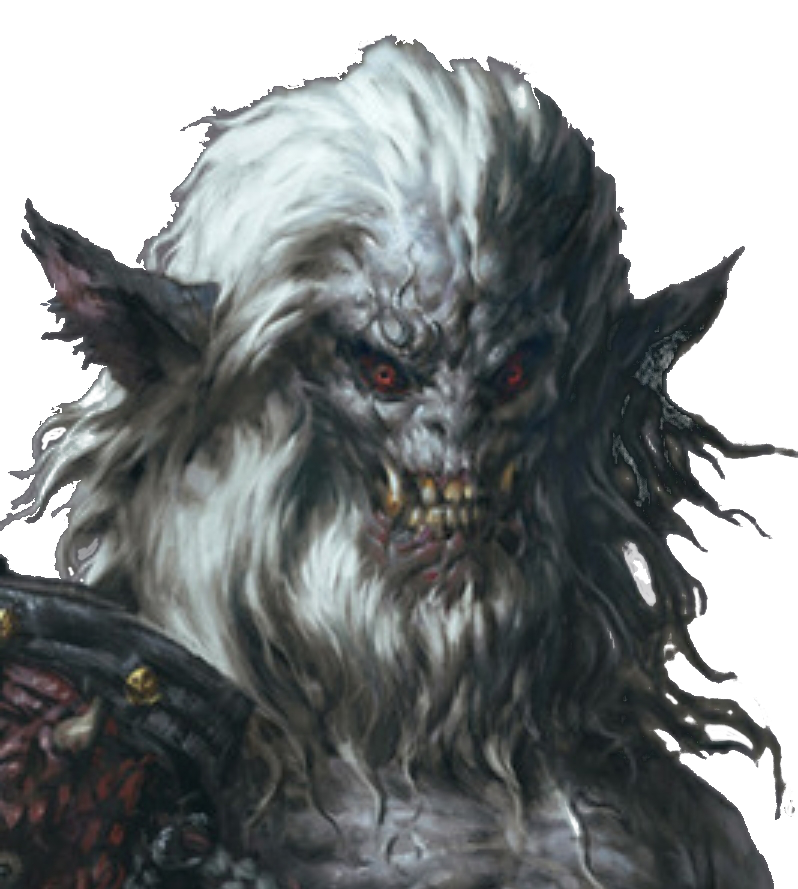
\includegraphics[width=0.7\textwidth]{img/dist/quaggoth.png}
			\caption{Quaggoth\label{fig:quaggoth}}
		\end{figure}
		Quaggoths are humanoids with long, shaggy, white hair covering their entire bodies that typically stand between 5'6" and 7' tall and can weigh as much as 300lb. Though their origin is, as yet, unknown, there has been much speculation on the matter. Many believe them to have been bred by the Drow to serve as a slave race. Some sages claim that they were once a semi-civilized race that dominated much of the Underdark through conquest and ritual sacrifice, until the Drow, Duergar, and other races broke their power. Others have speculated they had some sort of civilization on the surface and were driven underground; this theory is supported by the quaggoths' hatred for surface-dwelling dwarves and elves.
	\end{paperbox}
\end{figure}

Just as perplexing was the case of the two Drow Elves interred with the other captives. Seemingly, the two had run afoul of their own kind, and were handling it much differently from one another. One could be seen every day without fail standing near the cell's entrance, typically clutching and the bars or pacing nervously, and always muttering to himself things such as "I am NOT guilty!" and "I did not do it!" While one Drow seemed desperate to convince an unseen conversational partner of his innocence, the other took to his imprisonment with apparent cool indifference, and had been standing against a wall for nearly as long as Dox and Jhank had been present in the cell. Somehow, the calmer Drow had found a ruddy ruby, which he could be seen examining and polishing for many an hour. Though unfriendly, the Drow were not shy, and the one with the jewel had given his name to an inquiring captive as "Danixoth".\\

Today, a trio of new prisoners had been thrown in with the rest. One was a Wood Elf who introduced himself as Adran Oakenhill, and was covered with an amount of dirt that unsettlingly looked as though it predated his capture. Another was a Kenku who identified himself as "Alchemist" - though whether that was his name or profession was anyone's guess - and seemed to get along well with one or two prisoners but avoided the others entirely. Finally, a Tiefling was among them, and had spent his time since arriving in a mixture of meditation and smashing rocks together; he seemed bored.\\

Aside from these, the cell was also populated by a scattering of other characters. There was a pair of Underdeep Gnomes that appeared to be twins and talked to each other but never anyone else. Somewhat near the twins was a ragged and gaunt figure in tattered robes that might have been a dwarf if not for his gray skin, slight frame and diminutive stature (even by dwarven standards). There was also a purple-skinned man who, though covered in repulsive grime and muck, was quite friendly and forever attempted to engage his cell-mates in games of chance. From him, both Alchemist and Danixoth had won a small number of gold coins in wagers.\\

All told, the captives had amassed a small supply of possibly useful items. Dox took note of the ones he knew about.

\begin{dndtable}[lX]
	{\large Item} & {\large Owner}\\
	Crossbow Bolt & Dox\\
	Rusty Iron Bar & Jhank\\
	Dull Ruby & Danixoth\\
	Gold Pieces & Danixoth and Alchemist\\
	Rope Woven from Spider Webbing & Adran Oakenheel\\
	Shard of Flint & the Tiefling
\end{dndtable}

By comparing stories of their capture, the prisoners deduced that they had been drugged. As they were discussing this, a somewhat large tarantula hesitantly approached Jurnthar, seeming passive and as friendly as an arachnid can. Jurnthar whistled to the creature and extends a friendly hand, and it initially recoiled, but was soon coaxed to a perch on the dwarf's shoulder.\\

No longer able to withstand his frustration, Jhank rose to his feet and approached the Drow still clutching at his prison's bars. "What brought you here, captured by your own people?" he demanded. The Drow turned to face Jhank and looked him up and down as a sneer sprawled across his face.\\

% \begin{wrapfigure}{L}{0.5\linewidth}
% 	\centering
% 	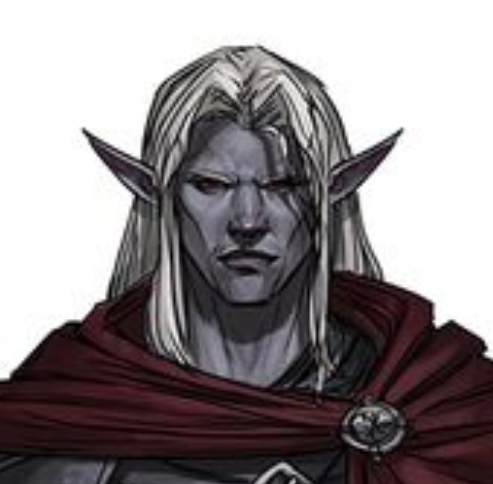
\includegraphics[width=0.7\linewidth]{img/dist/carith.png}
% 	\caption{Carith\label{fig:carith}}
% \end{wrapfigure}

"You have no place speaking to me, animal." The Drow spat out that last word, as though it could possibly have been mistaken as anything but a grave insult. He then turned his back to Jhank and resumed his routine of grabbing at the bars.\\

Dox, having heard this exchange, approached the pair by the door. The Drow noticed this and seemed to regard the half-Elf with considerably less disdain than the Lizardman. His expression quickly changed, however from one of mild interest to one of shock and disgust, as Dox slapped him hard across the face and warned him "Don't call him that." Jhank then grabbed his left hand in his own reptilian claw, balling it up into a fist before enclosing it with his other hand. With the implied threat in place, Jhank asked again: "Why are you here?".\\

The Drow coldly replied "I will not be threatened by a beast."\\

The two were not willing to harm the man for this information, and were about to back off when the Tiefling approached.\\
"Alright now, we're all in here together. No sense doing the guards' work for them."\\
The Drow, hearing the sense in his words, calmed down enough to apologize.\\
"I'm sorry, I'm just frustrated, I don't belong in here you see; I'm innocent."\\
The Tiefling nods sympathetically.\\
"We're all in that situation, just let's all help each other, yeah? I know we don't know you, but we're just trying to help. Let's work together."\\
"I'm sorry, you're right I need to calm down..."\\
The Drow then walked away from the group, bumping hard into Jhank on the way - though he only bounced off as though he had run into a brick wall, while Jhank remained unmoved.\\
The Tiefling then extended a hand toward Jhank, with the introduction: "Well met, I'm Nithe." Jhank did not shake his hand, but responded "I'm Jhank."\\
Nithe turned his unshaken hand toward Dox, who took it and said only "Evenwood".\\

Meanwhile, some prisoners were congregating near the strange mushroom man. Alchemist, the Kenku, gathered his spiritual essence and attempted to tap into the primordial forces that weave the fabric of reality in order to gain insight into the creature's land of origin, and information about its species. Unfortunately, that's not really how such things work, and nothing of the diminutive creature's mysterious nature was miraculously revealed to him\footnote{He asked to roll History to try to divine Stool's history/its people's history.}. Danixoth also attempted to gain information from it, in a much more reasonable and mundane way.\\
"Hey buddy, I don't mean to intrude, I know you don't like talking to us, but I was wondering - What's your name?"\\
"M-m-my name is Stool..." came the timid response. The creature had pressed itself back into the corner as far as it could go.\\
{\centering
	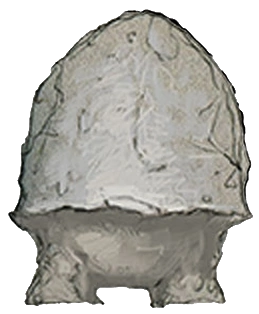
\includegraphics[width=0.2\textwidth]{img/dist/stool.png}
	\captionof{figure}{Stool\label{fig:stool}}
}

The purple man approached Alchemist, interrupting his reverie, and offered a bet: "I bet you that Drow dies by morning, care to take that action?", jabbing a gnarled thumb over his shoulder at Danixoth. Alchemist replied "How about something more interesting, I bet that if the orc and quaggoth could be made to fight, the quaggoth would handily win. Say, three gold pieces?"\\
"Done"\\

The purple man sidled up to the orc. "Hey fuckhead, that guy said you fuck goats," he said, pointing at the quaggoth. The orc's eyes widened and he charged the quaggoth and began screaming about how it would dismember it, but the quaggoth only protested "No sir, I did nothing of the sort, and I mean you no harm."\\
{
	\centering
	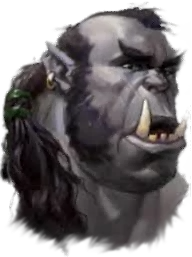
\includegraphics[width=0.2\textwidth]{img/dist/orc-prisoner.png}
	\captionof{figure}{Orc Prisoner\label{fig:orcPrisoner}}
}

There was then a clamoring from outside the cell, as two guards approached and barked out "No fighting!". The orc rounded on the guards and bellowed "Why don't you get in here and try to stop me!" to which the guards responded by drawing their crossbows and warning the orc to back off. He didn't listen, however, and the guards opened fire. One bolt lodged itself in his shoulder while the other slammed into his leg. The orc stumbled to a halt, lurched forward one more step and crashed to the	 ground, unconscious. The Drow reloaded and warned Jhank, Nithe and Dox to retreat from their position by the door as two quaggoth appeared from behind them. One Drow entered the cell alongside the qaggoth to drag the orc out and away into the hallway.\\

Alchemist remarked to the purple man "I guess our bet's off".\\

The quaggoth prisoner approached the Alchemist and the purple man and protested "I never said that, why did you say I said that?!?" but the purple man just laughed and walked away, flipping a coin in his hand.\\

Alchemist simply walked away wordlessly toward the fish man, and squatted down near him, mimicking his low growling noises. The creature's eyes snapped open with an agility that was unexpected for a beast of his size, startling Alchemist a bit, but he quickly recovered and the two recommenced gurgling at one another. Alchemist turned around and asked Jhank, "Hey, you look weird, he looks weird, do you guys know each other?" Jhank merely scoffed and turned away, but the fish man spoke "Do you wish to be awakened?"\\
	{\centering
	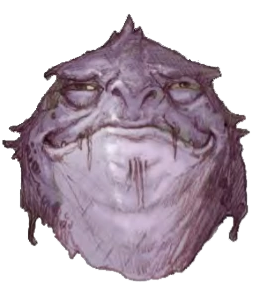
\includegraphics[width=0.5\linewidth]{img/dist/fish_man.png}
	\captionof{figure}{Fish-man\label{fig:fishman}}}
Alchemist returned his attention to the fish man before him and asked "In what way?"\\
"Violence is a circle, I represent peace"\\
"Okay, so how do I 'awaken'?"\\
"Join me on my path of peace, we can better this world"\\
"Actually, I'm good"\\
The fish man appeared unfazed by Alchemist's lack of interest.\\

Interested by his unusual manner of speech for a quaggoth, Dox intercepted it on its dejected walk to the back of the cavern and inquired, "Hey, you seem... different than the other quaggoth; how'd you wind up in here?"\\
The beast turned its head, seeming enthusiastic that someone was speaking to it without hostility. "Ah yes, my appearance. You see, I'm actually an elf, who was cursed to look like a quaggoth. My name is Darandil, I'm a prince from the Nelandril forest."

Jurnthar approaches the thin, dwarf-like man and asked "How's it going, brother?", mistaking him for a dwarf. "A lot better now that that filthy orc isn't in here anymore"
"I see you got a lot of tribal tatoos, friend, what's up with that? My name's Jurnthar, by the way."
"I am Wedgrar Greckan Warriors, my tribe were hunting stinkin' orcs like that when I was captured."
"What manner of fighter are you?"
"I cleave"
"Sounds like we'd make a good team; I shoot. These others appear"
"Whatever gets me to Grontilgrim"
"I hear that. When we get there I'll buy you a flagon of mead"
"Aye, and one for you too"
"It's good to meet a fellow dwarf in here"

Dox approaches the quaggoth and asked "Hail. How is it that you are in here"

Ah yes, my appearance. You see, I'm actually an elf. My name's Darandil a prince from the Nelandril forest.
That sucks.
Quite.

Danixoth approaches the other Drow and says "I can see by your clothing that you are not low-born, how came you here?"
"Another Drow, thank god. Are you from Menzobaranzan?"
"No, but I am familiar with the area."
"I had to run, and these guards - knowing what I am accused of - want to sacrifice me to Lolth. But I am innocent"
"I too, am fleeing false persecution. Do you have any plan to escape? I see you at the bars mumbling sometimes, is that part of a plan?"
"It's the only thing I can think to do. I'm a Drow, surely I deserve a trial?"
"Don't we all"

Adran examines the etchings on the ceiling, and notices that they glow a bit. Not enough to cast light in the cell, but just enough to be noticeable. Danixoth notices that they have no Lolth religious significance, and Adran senses some amount of magic emnating from the runes. 

Nithe meditates to attempt to commune with Bahamut.

Jurnthar approaches Adran and asked "What's your name, tree boy?" "Adran" "I'm Jurnthar. You're a shapeshifter, right?" "I am a druid, but I cannot yet shapeshift." "oh, I thought maybe you could turn into a spider" "I cannot" "Well if you ever need to, feel free to study my spider" "Actually I was hoping to get a sample of silk to compare to my rope" Jurnthar politely asked "Can we have some silk?" the tarantula blinks and poops some silk into Jurnthar's hand, which he then gives to Adran, who does nothing with it, which was weird. Jhank approaches the underdeep gnomes and asked "What's your deal?" from close up he could tell that one was male and the other female. The mail recoils and the female snaps "we don't talk to outsiders!", and Jhank retreats.

Dox pulls Jhank aside and lays out his plan "There's no way an orc that size was taken out by two non-lethal crossbow shots" and pulls out his strange-smelling bolt "I believe these to be coated" let's get 'em otay alchemist gets shut down yadda yadda

Danixoth approaches Nithe, who had finished meditating and asked "Did you catch that? Do you think we could help?" "I suggest we not let them get killed, and try not to draw attention" "let's get that shroom, dawg" "don't group up"

The other Drow approaches Alchemist and asked "Would you kindly remove yourself from my Stool's presence?" Alchemist wordlessly retreats back to the fish man, and the Drow and Stool appear to have a telepathic conversation.

Danixoth approaches and inquires "I forgot to get your name, sir" "My name is Carith Kzekarit" "I go by Danixoth. I see you know this mushroom. How far away can a mind be touched by it?" Carith explains that this creature is a Michonid that lost his name. He named it "Stool" because he used it as a seat. The spores, when clinging to a person, provided a telepathic communication channel within roughly 15 feet. Danixoth asked if Stool could be convinced to sit in a more central position. Carith glares at the mushroom, which moves to the center of the room and plops down onto the ground "Thank you" "Drow don't thank."

>spreads the plan to Jurnthar

>Jurnthar fills in his pal Wedgrar. The guard Drow clangs his sword against the cage and shouts out "Quiet down in there."

>Jhank fills in Darandil, who finds him fascinating

>Jhank signals that he's ready 

>spores get set up

>Jhank punches Darandil

>Diirka Deero

\chapter{2. Awake}


% For more columns, you can say \begin{dndtable}[your options here].
% For instance, if you wanted three columns, you could say
% \begin{dndtable}[XXX]. The usual host of tabular parameters are
% available as well.
% \begin{dndtable}[lX]
%    	\textbf{Item}  & \textbf{Owner} \\
%    	Crossbow bolt  & Evenwood \\
%    	Metal bar  & Jhank
% \end{dndtable}

% % You can optionally not include the background by saying
% % begin{monsterboxnobg}
% \begin{monsterbox}{Monster Foo}
% 	\textit{Small metasyntactic variable (goblinoid), neutral evil}\\
% 	\hline%
% 	\basics[%
% 	armorclass = 12,
% 	hitpoints  = \dice{3d8 + 3},
% 	speed      = 50 ft
% 	]
% 	\hline%
% 	\stats[
%     STR = \stat{12}, % This stat command will autocomplete the modifier for you
%     DEX = \stat{7}
% 	]
% 	\hline%
% 	\details[%
% 	% If you want to use commas in these sections, enclose the
% 	% description in braces.
% 	% I'm so sorry.
% 	languages = {Common Lisp, Erlang},
% 	]
% 	\hline \\[1mm]
% 	\begin{monsteraction}[Monster-super-powers]
% 		This Monster has some serious superpowers!
% 	\end{monsteraction}
% 	\monstersection{Actions}
% 	\begin{monsteraction}[Generate text]
% 		This one can generate tremendous amounts of text! Though only when it wants to.
% 	\end{monsteraction}

% 	\begin{monsteraction}[More actions]
%     See, here he goes again! Yet more text.
% 	\end{monsteraction}
% \end{monsterbox}

% \section{Spells}

% \begin{spell}
% 	{Beautiful Typesetting}
% 	{4th-level illusion}
% 	{1 action}
% 	{5 feet}
% 	{S, M (ink and parchment, which the spell consumes)}
% 	{Until dispelled}
% 	You are able to transform a written message of any length into a beautiful scroll. All creatures within range that can see the scroll must make a wisdom saving throw or be charmed by you until the spell ends.

% 	While the creature is charmed by you, they cannot take their eyes off the scroll and cannot willingly move away from the scroll. Also, the targets can make a wisdom saving throw at the end of each of their turns. On a success, they are no longer charmed.
% \end{spell}

% \section{Colors}

% This package provides several global color variables to style \lstinline!commentbox!, \lstinline!quotebox!, \lstinline!paperbox!, and \lstinline!dndtable! environments.

% \begin{dndtable}[lX]
%   \textbf{Color}         & \textbf{Description} \\
%   \lstinline!commentboxcolor! & Controls \lstinline!commentbox! background. \\
%   \lstinline!paperboxcolor!   & Controls \lstinline!paperbox! background. \\
%   \lstinline!quoteboxcolor!   & Controls \lstinline!quotebox! background. \\
%   \lstinline!tablecolor!      & Controls background of even \lstinline!dndtable! rows. \\
% \end{dndtable}

% See Table~\ref{tab:colors} for a list of accent colors that match the core books.

% \begin{table*}
%   \begin{dndtable}[XX]
%     \textbf{Color}                            & \textbf{Description} \\
%     \lstinline!PhbLightGreen!                      & {\color{PhbLightGreen} Light green used in PHB Part 1} \\
%     \lstinline!PhbLightCyan!                       & {\color{PhbLightCyan} Light cyan used in PHB Part 2} \\
%     \lstinline!PhbMauve!                           & {\color{PhbMauve} Pale purple used in PHB Part 3} \\
%     \lstinline!PhbTan!                             & {\color{PhbTan} Light brown used in PHB appendix} \\
%     \lstinline!DmgLavender!                        & {\color{DmgLavender} Pale purple used in DMG Part 1} \\
%     \lstinline!DmgCoral!                           & {\color{DmgCoral} Orange-pink used in DMG Part 2} \\
%     \lstinline!DmgSlateGray! (\lstinline!DmgSlateGrey!) & {\color{DmgSlateGray} Blue-gray used in PHB Part 3} \\
%     \lstinline!DmgLilac!                           & {\color{DmgLilac} Purple-gray used in DMG appendix} \\
%   \end{dndtable}
%   \caption{Colors supported by this package}%
%   \label{tab:colors}
% \end{table*}

\end{document}